\documentclass[UTF8,a4paper,11pt]{ctexart}

\usepackage{amsmath,amssymb,bm}
\usepackage{booktabs}
\usepackage{geometry}
\usepackage{hyperref}
\usepackage{xcolor}
\usepackage{enumitem}
\usepackage{caption}
\usepackage{float}
\usepackage{graphicx}
\usepackage{tikz}
\usepackage{pgfplots}
\usetikzlibrary{arrows.meta,backgrounds,calc,decorations.pathreplacing,fit,matrix,positioning,shapes.geometric}
\pgfplotsset{compat=1.18}

\geometry{left=2.35cm,right=2.35cm,top=2.45cm,bottom=2.45cm}
\hypersetup{colorlinks=true,linkcolor=blue!55!black,urlcolor=blue!65!black,citecolor=blue!55!black}
\setlength{\parindent}{2em}
\setlength{\parskip}{0.22em}
\setlength{\emergencystretch}{1em}
\setlist{nosep}

\newcommand{\qca}{量子点元胞自动机（QCA）}
\newcommand{\Ek}{E_{k}^{ij}}
\newcommand{\pending}{\texttt{RESULT\_PENDING}}
\newcommand{\csr}{\textsc{CSR}}
\tikzset{
  block/.style={draw,rounded corners=2pt,thick,align=center,minimum height=9mm,
                text width=29mm,fill=blue!7},
  compile/.style={block,fill=cyan!10,draw=cyan!55!black},
  bistable/.style={block,fill=orange!11,draw=orange!72!black},
  coherence/.style={block,fill=violet!9,draw=violet!65!black},
  guard/.style={block,fill=green!10,draw=green!55!black},
  io/.style={block,fill=gray!9,draw=gray!65},
  arrow/.style={-{Latex[length=2.2mm]},thick,draw=gray!78!black},
  stage/.style={draw,dashed,rounded corners=3pt,inner sep=5pt},
  cell/.style={circle,draw,thick,minimum size=7.5mm,inner sep=0pt,fill=white}
}

\title{Bistable与Coherence-vector QCA仿真的严格等价稀疏编译加速\\
\large 第六章时钟分区与局部耦合思想的物理内核实现}
\author{iFCN仿真模块技术与SCI写作草案}
\date{\today}

\begin{document}
\maketitle

\begin{abstract}
本文给出一种面向双稳态（Bistable）和相干矢量（Coherence-vector）QCA仿真的严格等价加速框架。方法不引入训练模型，也不以近似函数替换物理方程，而是把论文第六章中的时钟分区、局部耦合和重复结构思想转化为一次性物理内核编译：采用保持基准遍历顺序的空间桶生成有效元胞对，将邻居状态引用与扭结能压缩为行内有序的\csr{}式耦合记录，并把可更新元胞及其时钟区元数据编译为连续记录。Bistable内核保持有种子随机序列驱动的Gauss--Seidel更新、收敛阈值和非线性响应不变；Coherence-vector内核保持稳态初始化、Euler或既有分量式Runge--Kutta路径不变，同时缓存四相$\Gamma$序列并复用\texttt{hypot}/\texttt{tanh}公共子表达式。由于候选筛选只删除必然超出作用半径的元胞对，且每行的邻居、浮点累加和状态更新顺序均与基准实现一致，可通过对执行轨迹的归纳证明建立数值等价性。开发阶段已覆盖61个唯一QCA版图：36个iFCN版图的交叉冒烟测试及25个hfut-sim版图的较长预实验均无逻辑或数值误差。hfut-sim预实验的Bistable与Coherence-vector（Euler）套件加速比分别为$1.9462\times$和$2.2568\times$；Coherence使用缩短的40960步非默认协议，故这些数据只作为工程预证据，30次以上的正式重复统计仍标为\pending。框架还通过GUI自动临时QCA快照消除“布局布线结果必须先手工保存才能仿真”的限制。
\end{abstract}

\noindent\textbf{关键词：}QCA；双稳态仿真；相干矢量仿真；稀疏编译；严格等价；Gauss--Seidel；连续内存

\section{研究问题与范围}

本文只研究两类物理仿真器的加速：Bistable功能仿真和Coherence-vector动态仿真。目标不是得到一条“看起来像方波”的近似输出，而是在相同布局、输入、物理参数、采样数、随机种子、积分方法和编译环境下，保持基准引擎的离散执行语义，并减少重复建图、指针追踪、时钟求值和公共数学函数开销。

设布局含$N$个元胞，有效作用半径为$r_e$，半径内的有向耦合边数为$M$，采样点数为$T$。Bistable在每个采样点平均执行$I$轮固定点迭代；Coherence-vector每步使用$s$次斜率求值（Euler时$s=1$，既有分量式Runge--Kutta路径时$s=4$）。旧实现的主要代价包括
\begin{equation}
  C_{\mathrm{old}}
  =\underbrace{\Theta(N^2 C_k)}_{\text{全对全距离与扭结能建图}}
  +\underbrace{\Theta(TIM)}_{\text{Bistable}}
  \quad\text{或}\quad
  \underbrace{\Theta(TsM)}_{\text{Coherence-vector}},
\end{equation}
其中$C_k$表示一次元胞对静电能计算的常数开销。运行期的大$O$阶不一定改变，但稀疏编译显著降低一次性建图代价和循环常数；这也是本文对性能结论采取实测而非夸大渐近复杂度的原因。

\section{从第六章思想到严格物理内核}

第六章的核心观察是：QCA相互作用具有有限局部性，四相时钟又使元胞按区域重复使用相同控制量。这两点可以直接用于编译物理仿真器，而不必改写元胞响应方程。图~\ref{fig:framework}从候选检查和内存访问两个层面比较基准机制与本文机制。

\begin{figure}[H]
\centering
\resizebox{\linewidth}{!}{%
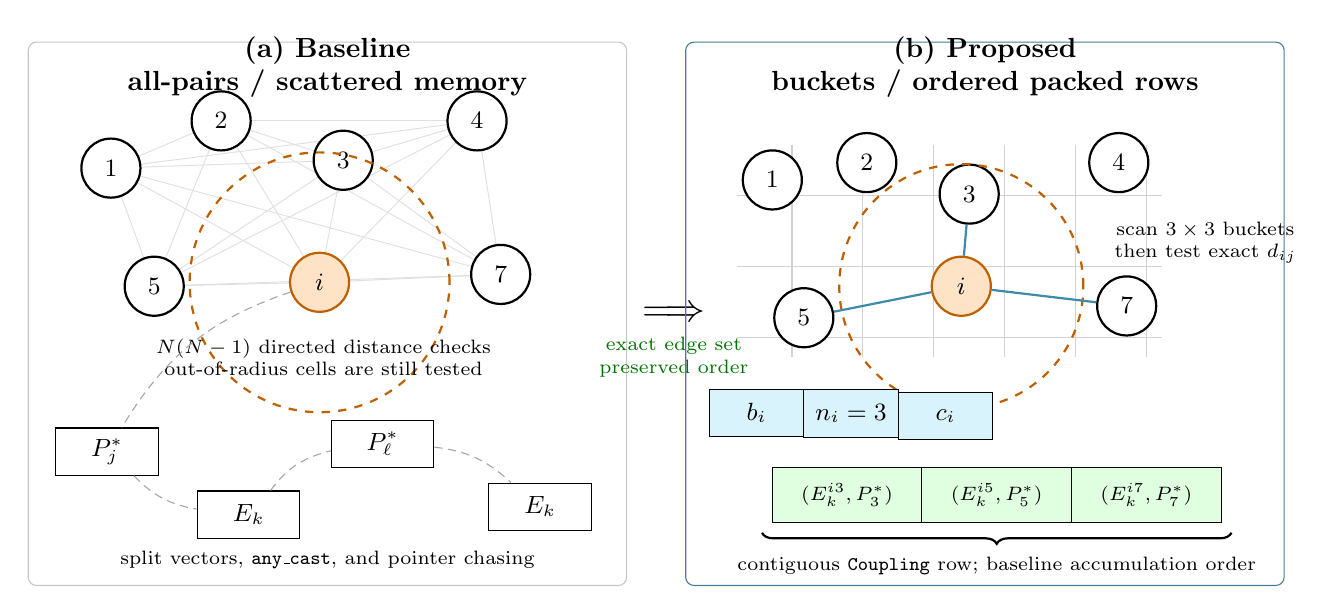
\begin{tikzpicture}[font=\small]
  % Legacy panel: all-pairs candidates and fragmented hot-loop storage.
  \begin{scope}
    \draw[rounded corners=3pt,gray!45] (-.45,-1.35) rectangle (7.15,5.55);
    \node[font=\bfseries,align=center] at (3.35,5.23)
      {(a) Baseline\\all-pairs / scattered memory};
    \coordinate (la) at (.6,3.95);
    \coordinate (lb) at (2.0,4.55);
    \coordinate (lc) at (3.55,4.05);
    \coordinate (ld) at (5.25,4.55);
    \coordinate (le) at (1.15,2.45);
    \coordinate (lf) at (3.25,2.50);
    \coordinate (lg) at (5.55,2.60);
    \foreach \u/\v in {la/lb,la/lc,la/ld,la/le,la/lf,la/lg,
      lb/lc,lb/ld,lb/le,lb/lf,lb/lg,lc/ld,lc/le,lc/lf,lc/lg,
      ld/le,ld/lf,ld/lg,le/lf,le/lg,lf/lg}
      \draw[gray!24,line width=.35pt] (\u)--(\v);
    \node[cell] (L1) at (la) {$1$};
    \node[cell] (L2) at (lb) {$2$};
    \node[cell] (L3) at (lc) {$3$};
    \node[cell] (L4) at (ld) {$4$};
    \node[cell] (L5) at (le) {$5$};
    \node[cell,fill=orange!22,draw=orange!75!black] (Li) at (lf) {$i$};
    \node[cell] (L7) at (lg) {$7$};
    \draw[dashed,orange!75!black,thick] (Li) circle (1.65);
    \node[font=\scriptsize,align=center] at (3.3,1.55)
      {$N(N-1)$ directed distance checks\\out-of-radius cells are still tested};
    \node[draw,minimum width=13mm,minimum height=6mm] (m1) at (.55,.35) {$P_j^\ast$};
    \node[draw,minimum width=13mm,minimum height=6mm] (m2) at (2.35,-.45) {$E_k$};
    \node[draw,minimum width=13mm,minimum height=6mm] (m3) at (4.05,.45) {$P_\ell^\ast$};
    \node[draw,minimum width=13mm,minimum height=6mm] (m4) at (6.05,-.35) {$E_k$};
    \draw[densely dashed,gray!70] (Li) to[bend right=20] (m1);
    \draw[densely dashed,gray!70] (m1) to[bend right=18] (m2);
    \draw[densely dashed,gray!70] (m2) to[bend left=20] (m3);
    \draw[densely dashed,gray!70] (m3) to[bend left=18] (m4);
    \node[font=\scriptsize] at (3.35,-1.02)
      {split vectors, \texttt{any\_cast}, and pointer chasing};
  \end{scope}

  \node[font=\Large] at (7.75,2.1) {$\Longrightarrow$};
  \node[font=\scriptsize,align=center,text=green!45!black] at (7.75,1.55)
    {exact edge set\\preserved order};

  % Proposed panel: bucket candidates and packed row storage.
  \begin{scope}[xshift=8.35cm]
    \draw[rounded corners=3pt,cyan!55!black] (-.45,-1.35) rectangle (7.15,5.55);
    \node[font=\bfseries,align=center] at (3.35,5.23)
      {(b) Proposed\\buckets / ordered packed rows};
    \draw[step=.9cm,gray!35] (.2,1.55) grid (5.6,4.25);
    \node[cell] (R1) at (.65,3.80) {$1$};
    \node[cell] (R2) at (1.85,4.02) {$2$};
    \node[cell] (R3) at (3.15,3.62) {$3$};
    \node[cell] (R4) at (5.05,4.02) {$4$};
    \node[cell] (R5) at (1.05,2.05) {$5$};
    \node[cell,fill=orange!22,draw=orange!75!black] (Ri) at (3.05,2.45) {$i$};
    \node[cell] (R7) at (5.15,2.20) {$7$};
    \draw[dashed,orange!75!black,thick] (Ri) circle (1.55);
    \draw[thick,cyan!65!black] (Ri)--(R3);
    \draw[thick,cyan!65!black] (Ri)--(R5);
    \draw[thick,cyan!65!black] (Ri)--(R7);
    \node[font=\scriptsize,align=center] at (6.15,3.0)
      {scan $3\times3$ buckets\\then test exact $d_{ij}$};

    \matrix (meta) at (1.65,.82) [matrix of nodes,ampersand replacement=\&,
      nodes={draw,minimum height=6mm,minimum width=12mm},
      column sep=-\pgflinewidth] {
      |[fill=cyan!15]| $b_i$ \& |[fill=cyan!15]| $n_i=3$ \& |[fill=cyan!15]| $c_i$ \\
    };
    \matrix (band) at (3.5,-.20) [matrix of nodes,ampersand replacement=\&,
      nodes={draw,minimum height=7mm,minimum width=19mm,font=\scriptsize},
      column sep=-\pgflinewidth] {
      |[fill=green!12]| $(E_k^{i3},P_3^\ast)$ \&
      |[fill=green!12]| $(E_k^{i5},P_5^\ast)$ \&
      |[fill=green!12]| $(E_k^{i7},P_7^\ast)$ \\
    };
    \draw[decorate,decoration={brace,mirror,amplitude=4pt},thick]
      (band.south west) -- (band.south east)
      node[midway,below=5pt,font=\scriptsize]
      {contiguous \texttt{Coupling} row; baseline accumulation order};
  \end{scope}
\end{tikzpicture}
}
\caption{基准与本文稀疏编译机制对比。空间桶只减少不可能命中的候选检查；精确半径判定、有效边集合及行内顺序保持不变。}
\label{fig:framework}
\end{figure}

这种转换包含三条原则：
\begin{enumerate}
  \item \textbf{局部性用于删减候选，不用于删减有效耦合。}空间桶只排除不可能满足$d_{ij}\le r_e$的元胞对，最终仍执行与基准相同的三维距离判断；
  \item \textbf{时钟分区用于共享控制量，不用于冻结元胞。}同一时钟区的元胞共享$\Gamma_c(t)$缓存，但每个元胞仍在每个规定采样点更新；
  \item \textbf{连续化用于减少访存，不用于重排算术。}\csr{}行内邻居按基准遍历序保存，点积仍按相同顺序累加。
\end{enumerate}

\section{一次性有序稀疏编译}

\subsection{扭结能图}

对元胞$i$与$j$，用三维中心距离
\begin{equation}
 d_{ij}=\sqrt{(x_i-x_j)^2+(y_i-y_j)^2+
 \bigl((\ell_i-\ell_j)h_\ell\bigr)^2}
\end{equation}
判断是否满足$d_{ij}\le r_e$。若满足，则按四量子点电荷模型计算扭结能
\begin{equation}
 E_k^{ij}=E_{\mathrm{different}}^{ij}-E_{\mathrm{same}}^{ij}.
\end{equation}
工程中的\csr{}式编译结果由两类连续记录组成：
\begin{align}
 \texttt{PreparedCell}_i&=\{b_i,n_i,c_i,P_i^\ast,\ldots\},\\
 \texttt{Coupling}[q]&=\{E_k(q),P_{\mathrm{nbr}(q)}^\ast\},
 \qquad q=0,\ldots,M-1,
\end{align}
其中$b_i$和$n_i$分别是元胞$i$在全局耦合带中的起点与长度，$c_i$为时钟区，$P^\ast$为直接状态引用。故第$i$行对应$[b_i,b_i+n_i)$。这种“行元数据+连续耦合带”在逻辑上等价于\csr{}，但没有虚构实现中不存在的整数\texttt{col\_idx}数组。

\subsection{保持顺序的空间桶}

桶边长取不小于$r_e$。元胞仅在本桶及三维相邻桶中寻找候选，然后再次执行精确距离判断。为了保持浮点执行轨迹，候选的发现顺序不能直接成为\csr{}顺序；每行候选必须按基准布局序号稳定排序，随后才计算并写入扭结能。图~\ref{fig:bucket-csr}展示这一过程。

\begin{figure}[H]
\centering
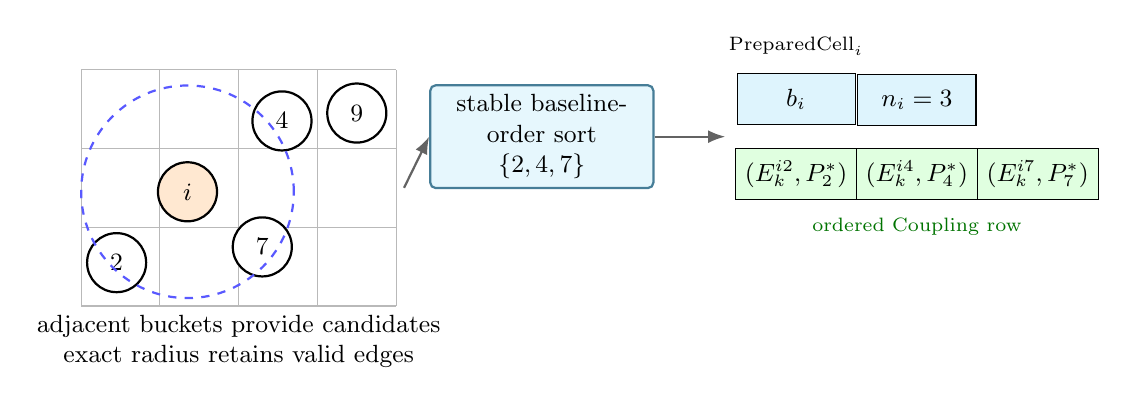
\begin{tikzpicture}[font=\small,node distance=8mm]
  \draw[step=10mm,gray!55] (0,0) grid (4,3);
  \node[cell,fill=orange!18] (a) at (1.35,1.45) {$i$};
  \node[cell] (b) at (.45,.55) {$2$};
  \node[cell] (c) at (2.30,.75) {$7$};
  \node[cell] (d) at (2.55,2.35) {$4$};
  \node[cell] (e) at (3.50,2.45) {$9$};
  \draw[dashed,blue!65,thick] (a) circle (1.35);
  \node[align=center] at (2,-.45)
    {adjacent buckets provide candidates\\exact radius retains valid edges};

  \node[compile,text width=26mm] (sort) at (5.85,2.15)
    {stable baseline-order sort\\$\{2,4,7\}$};
  \draw[arrow] (4.1,1.5)--(sort.west);

  \matrix (m) [matrix of nodes,nodes={draw,minimum height=6.5mm,minimum width=15mm},
                column sep=-\pgflinewidth,row sep=2mm,right=9mm of sort] {
    |[fill=cyan!13]| $b_i$ & |[fill=cyan!13]| $n_i=3$ & |[draw=none]| \\
    |[fill=green!12]| $(E_k^{i2},P_2^\ast)$ &
    |[fill=green!12]| $(E_k^{i4},P_4^\ast)$ &
    |[fill=green!12]| $(E_k^{i7},P_7^\ast)$ \\
  };
  \node[above=1mm of m-1-1,font=\scriptsize] {$\mathrm{PreparedCell}_i$};
  \node[below=1mm of m-2-2,font=\scriptsize,text=green!45!black]
    {ordered Coupling row};
  \draw[arrow] (sort.east)--(m.west);
\end{tikzpicture}
\caption{空间桶到行内有序\csr{}的编译。图中编号表示基准布局遍历序号，而非空间桶发现顺序。}
\label{fig:bucket-csr}
\end{figure}

若布局密度受限，每个桶平均含$\bar b$个元胞，则候选扫描约为$\mathcal O(N\bar b)$，有效边计算为$\mathcal O(M)$。稳定恢复顺序的代价取决于每行候选数，可写为$\mathcal O(\sum_i d_i\log d_i)$；由于$d_i$通常远小于$N$，它显著小于全对全建图。若极端布局把所有元胞放入同一桶，最坏情况仍退化为$\Theta(N^2)$，但不会损失正确性。

\section{Bistable严格等价加速}

\subsection{基准方程}

元胞$i$在采样点$j$的局部场为
\begin{equation}
 H_i^{(j)}=\sum_{q=b_i}^{b_i+n_i-1}
   \texttt{Coupling}[q].E_k\,
   \bigl(*\texttt{Coupling}[q].P^\ast\bigr),
\end{equation}
其无量纲响应变量和极化更新为
\begin{align}
 u_i^{(j)}&=\frac{H_i^{(j)}}{2\Gamma_{c_i}^{(j)}},\\
 P_i^{(j)}&=f(u_i^{(j)})
  =\begin{cases}
  1,&u_i>1000,\\
 -1,&u_i<-1000,\\
  u_i,&|u_i|<10^{-3},\\
 \dfrac{u_i}{\sqrt{1+u_i^2}},&\text{其他情况}.
 \end{cases}
\end{align}
当一轮内所有可更新元胞均满足
\begin{equation}
 |P_{i,\mathrm{new}}-P_{i,\mathrm{old}}|\le\varepsilon_P
\end{equation}
时停止，否则最多执行$I_{\max}$轮。

\subsection{确定性Gauss--Seidel执行轨迹}

加速内核不改用Jacobi、不引入超松弛，也不并行更新相互依赖的元胞。每轮仍从层内自然序列执行\texttt{iota+shuffle}，并消费与基准后端相同的有种子随机数流；图中的调度带表示某一轮得到的确定序列，而不是预先固定所有轮次。更新$i$后，新$P_i$立即可被本轮后续元胞读取，因此仍是Gauss--Seidel语义。图~\ref{fig:gs}中的实线表示本轮已经写回的新值，虚线表示尚未更新的旧值。

\begin{figure}[H]
\centering
\resizebox{\linewidth}{!}{%
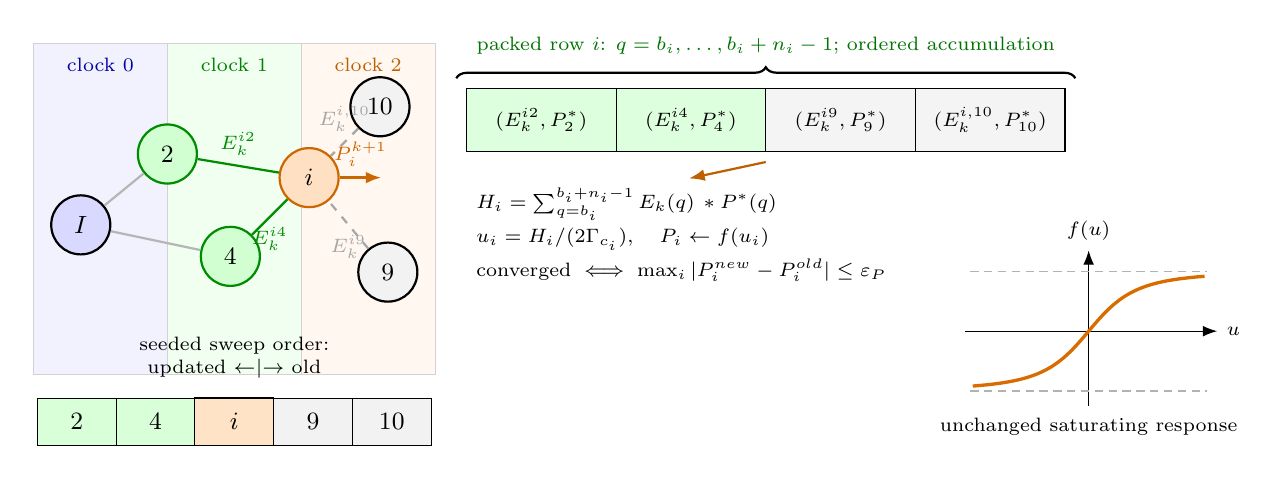
\begin{tikzpicture}[font=\small]
  % Clock-zone background and a local physical neighbourhood.
  \fill[blue!5] (-.15,.85) rectangle (1.55,5.05);
  \fill[green!6] (1.55,.85) rectangle (3.25,5.05);
  \fill[orange!6] (3.25,.85) rectangle (4.95,5.05);
  \draw[gray!35] (-.15,.85) rectangle (4.95,5.05);
  \draw[gray!35] (1.55,.85)--(1.55,5.05);
  \draw[gray!35] (3.25,.85)--(3.25,5.05);
  \node[font=\scriptsize,blue!65!black] at (.70,4.78) {clock 0};
  \node[font=\scriptsize,green!50!black] at (2.40,4.78) {clock 1};
  \node[font=\scriptsize,orange!75!black] at (4.10,4.78) {clock 2};

  \node[cell,fill=blue!15] (in) at (.45,2.75) {$I$};
  \node[cell,fill=green!18,draw=green!55!black] (p2) at (1.55,3.65) {$2$};
  \node[cell,fill=green!18,draw=green!55!black] (p4) at (2.35,2.35) {$4$};
  \node[cell,fill=orange!24,draw=orange!80!black] (pi) at (3.35,3.35) {$i$};
  \node[cell,fill=gray!10] (p9) at (4.35,2.15) {$9$};
  \node[cell,fill=gray!10] (p10) at (4.25,4.25) {$10$};
  \draw[thick,gray!58] (in)--(p2);
  \draw[thick,gray!58] (in)--(p4);
  \draw[thick,green!55!black] (p2)--node[above,font=\scriptsize]{$E_k^{i2}$}(pi);
  \draw[thick,green!55!black] (p4)--node[below,font=\scriptsize]{$E_k^{i4}$}(pi);
  \draw[thick,dashed,gray!70] (p9)--node[below,font=\scriptsize]{$E_k^{i9}$}(pi);
  \draw[thick,dashed,gray!70] (p10)--node[above,font=\scriptsize]{$E_k^{i,10}$}(pi);
  \draw[-{Latex[length=2mm]},very thick,orange!80!black] (pi) -- ++(.92,0)
    node[midway,above,font=\scriptsize]{$P_i^{k+1}$};

  % The actual shuffled order for this sweep.
  \matrix (sched) at (2.40,.25) [matrix of nodes,ampersand replacement=\&,
    nodes={draw,minimum width=10mm,minimum height=6mm},
    column sep=-\pgflinewidth] {
    |[fill=green!15]| $2$ \& |[fill=green!15]| $4$ \&
    |[fill=orange!22]| $i$ \& |[fill=gray!10]| $9$ \& |[fill=gray!10]| $10$ \\
  };
  \node[font=\scriptsize,anchor=south,align=center,text width=46mm] at (sched.north)
    {seeded sweep order: updated $\leftarrow\mid\rightarrow$ old};

  % Packed row and exact accumulation.
  \matrix (row) at (9.15,4.08) [matrix of nodes,ampersand replacement=\&,
    nodes={draw,minimum width=19mm,minimum height=8mm,font=\scriptsize},
    column sep=-\pgflinewidth] {
    |[fill=green!13]| $(E_k^{i2},P_2^\ast)$ \&
    |[fill=green!13]| $(E_k^{i4},P_4^\ast)$ \&
    |[fill=gray!9]| $(E_k^{i9},P_9^\ast)$ \&
    |[fill=gray!9]| $(E_k^{i,10},P_{10}^\ast)$ \\
  };
  \draw[decorate,decoration={brace,amplitude=4pt},thick]
    (row.north west)--(row.north east)
    node[midway,above=5pt,font=\scriptsize,text=green!45!black]
      {packed row $i$: $q=b_i,\ldots,b_i+n_i-1$; ordered accumulation};

  \node[align=left,anchor=west,text width=54mm,font=\scriptsize] (eq) at (5.35,2.62)
    {$H_i=\sum_{q=b_i}^{b_i+n_i-1}E_k(q)\,*P^\ast(q)$\\[2pt]
     $u_i=H_i/(2\Gamma_{c_i}),\quad P_i\leftarrow f(u_i)$\\[2pt]
     $\mathrm{converged}\iff
       \max_i|P_i^{new}-P_i^{old}|\le\varepsilon_P$};
  \draw[-{Latex[length=2mm]},thick,orange!75!black] (row.south) -- (eq.north);

  % Nonlinear bistable response, shown as a mechanism rather than a box.
  \begin{scope}[xshift=13.25cm,yshift=1.40cm,xscale=.64,yscale=.76]
    \draw[-{Latex[length=1.8mm]}] (-2.45,0)--(2.55,0) node[right,font=\scriptsize]{$u$};
    \draw[-{Latex[length=1.8mm]}] (0,-1.25)--(0,1.35) node[above,font=\scriptsize]{$f(u)$};
    \draw[orange!85!black,very thick,domain=-2.3:2.3,samples=80]
      plot (\x,{\x/sqrt(1+\x*\x)});
    \draw[densely dashed,gray!60] (-2.35,1)--(2.35,1);
    \draw[densely dashed,gray!60] (-2.35,-1)--(2.35,-1);
    \node[font=\scriptsize,align=center] at (0,-1.60)
      {unchanged saturating response};
  \end{scope}
\end{tikzpicture}
}
\caption{Bistable稀疏内核的物理更新机制。空间邻接、行内耦合带和本轮随机次序共同确定严格同序的Gauss--Seidel原位传播。}
\label{fig:gs}
\end{figure}

运行期开销仍为$\mathcal O(TIM)$，但有四项常数优化：连续\texttt{Coupling}带的流式读取；直接极化引用消除热循环中的\texttt{any\_cast}；预编译动态元胞分类；每个元胞直接持有其时钟轨迹引用。若某电路的主要时间消耗来自极少元胞和极少迭代，一次编译成本可能抵消收益，因此论文必须同时报告冷启动和复用编译图两类时间。

\section{Coherence-vector严格等价加速}

\subsection{状态方程与稳态初始化}

定义局部耦合能$E_i=\sum_j E_k^{ij}P_j$、时钟隧穿能$\Gamma$以及
\begin{equation}
 \Omega_i=\frac{\operatorname{hypot}(2\Gamma,E_i)}{\hbar},\qquad
 \theta_i=\tanh\!\left(\frac{\hbar\Omega_i}{2k_BT}\right).
\end{equation}
稳态分量为
\begin{equation}
 \lambda_{x,i}^{ss}=\frac{2\Gamma}{\hbar\Omega_i}\theta_i,qquad
 \lambda_{y,i}^{ss}=0,qquad
 \lambda_{z,i}^{ss}=-\frac{E_i}{\hbar\Omega_i}\theta_i.
\end{equation}
在既有模型中，动态方程写为
\begin{align}
 \dot\lambda_x&=\frac{\lambda_x^{ss}-\lambda_x}{\tau}
                 -\frac{E_i\lambda_y}{\hbar},\\
 \dot\lambda_y&=\frac{E_i\lambda_x+2\Gamma\lambda_z}{\hbar}
                 -\frac{\lambda_y}{\tau},\\
 \dot\lambda_z&=\frac{-E_i\theta_i-\Omega_i(2\Gamma\tau\lambda_y+
                 \hbar\lambda_z)}{\tau\hbar\Omega_i}.
\end{align}
动态阶段的极化映射保持为$P_i=-\lambda_{z,i}$。加速版本不修改稳态迭代容差、最大迭代次数、时间步长，也不把Euler与既有分量式Runge--Kutta路径互相替换。后者是项目原有的$x/y/z$各分量阶段更新语义，并非完整耦合ODE的标准RK4；本文只严格复刻它，不宣称修正了积分方法。

\subsection{四相时钟缓存与公共子表达式融合}

对$c\in\{0,1,2,3\}$和$j\in[0,T)$，只把基准时钟发生器的结果缓存为
\begin{equation}
 \Gamma_{\mathrm{cache}}[j,c]=\Gamma_c(t_j),
 \qquad |\Gamma_{\mathrm{cache}}|=4T.
\end{equation}
$2\Gamma$及$2\Gamma/\hbar$没有单独预计算，而是在融合核中从当前$\Gamma$求得。输入发生器也可在内存预算允许时缓存；预算不足则回到原发生器，数值语义不变。
在每个元胞步内，$\Omega_i$与$\theta_i$只依赖当前$E_i$、$\Gamma$和温度，因此可由$x$、$y$、$z$三个斜率共享。Euler中每个元胞步只需求值一次公共核；既有分量式Runge--Kutta路径的各阶段也复用与该阶段无关的公共量。图~\ref{fig:coherence-fusion}显示从重复求值到融合核的转换。

\begin{figure}[H]
\centering
\resizebox{\linewidth}{!}{%
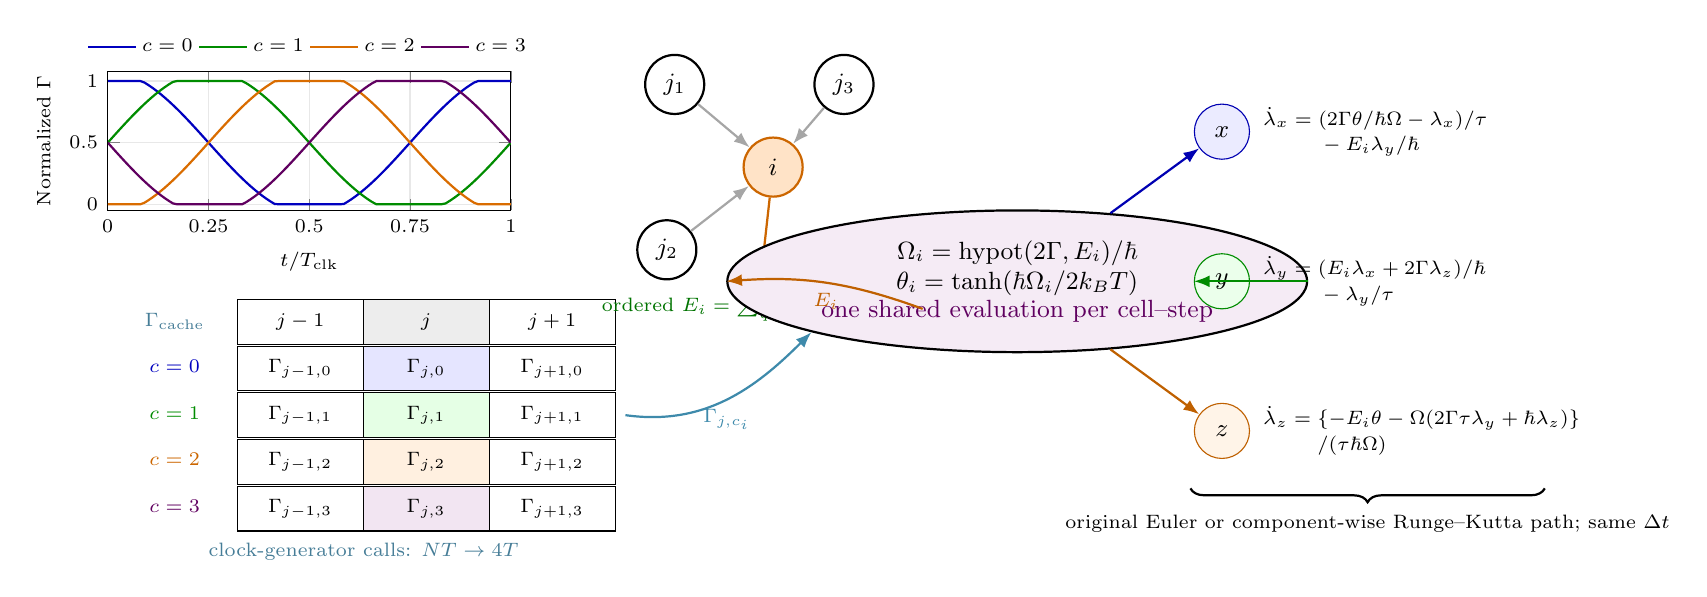
\begin{tikzpicture}[font=\small]
  % Four-phase clock curves.
  \begin{axis}[
    at={(0cm,4.15cm)},anchor=south west,
    width=6.7cm,height=3.35cm,
    xmin=0,xmax=1,ymin=-.05,ymax=1.08,
    xlabel={$t/T_{\mathrm{clk}}$},ylabel={Normalized $\Gamma$},
    xtick={0,.25,.5,.75,1},ytick={0,.5,1},
    grid=major,major grid style={gray!18},
    tick label style={font=\scriptsize},label style={font=\scriptsize},
    legend style={font=\scriptsize,draw=none,at={(.5,1.03)},anchor=south,legend columns=4}
  ]
    \addplot[blue!75!black,thick,domain=0:1,samples=100]
      {max(0,min(1,.5+.58*cos(deg(2*pi*x))))};
    \addplot[green!55!black,thick,domain=0:1,samples=100]
      {max(0,min(1,.5+.58*cos(deg(2*pi*x)-90)))};
    \addplot[orange!85!black,thick,domain=0:1,samples=100]
      {max(0,min(1,.5+.58*cos(deg(2*pi*x)-180)))};
    \addplot[violet!75!black,thick,domain=0:1,samples=100]
      {max(0,min(1,.5+.58*cos(deg(2*pi*x)-270)))};
    \legend{$c=0$,$c=1$,$c=2$,$c=3$}
  \end{axis}

  % Sample-major four-phase Gamma cache.
  \matrix (gcache) at (3.25,1.55) [matrix of nodes,ampersand replacement=\&,
    nodes={draw,minimum width=16mm,minimum height=5.7mm,font=\scriptsize},
    column sep=-\pgflinewidth,row sep=-\pgflinewidth] {
    |[text=cyan!55!black,draw=none]| $\Gamma_{\mathrm{cache}}$ \&
      $j-1$ \& |[fill=gray!14]| $j$ \& $j+1$ \\
    |[text=blue!75!black,draw=none]| $c=0$ \& $\Gamma_{j-1,0}$ \& |[fill=blue!10]| $\Gamma_{j,0}$ \& $\Gamma_{j+1,0}$ \\
    |[text=green!55!black,draw=none]| $c=1$ \& $\Gamma_{j-1,1}$ \& |[fill=green!10]| $\Gamma_{j,1}$ \& $\Gamma_{j+1,1}$ \\
    |[text=orange!80!black,draw=none]| $c=2$ \& $\Gamma_{j-1,2}$ \& |[fill=orange!12]| $\Gamma_{j,2}$ \& $\Gamma_{j+1,2}$ \\
    |[text=violet!75!black,draw=none]| $c=3$ \& $\Gamma_{j-1,3}$ \& |[fill=violet!10]| $\Gamma_{j,3}$ \& $\Gamma_{j+1,3}$ \\
  };
  \node[font=\scriptsize,text=cyan!55!black] at (3.25,-.18)
    {clock-generator calls: $NT\rightarrow4T$};

  % Local electrostatic field at one cell.
  \node[cell,fill=orange!22,draw=orange!80!black] (ci) at (8.45,4.70) {$i$};
  \node[cell] (n1) at (7.20,5.75) {$j_1$};
  \node[cell] (n2) at (7.10,3.65) {$j_2$};
  \node[cell] (n3) at (9.35,5.75) {$j_3$};
  \draw[-{Latex[length=2mm]},thick,gray!70] (n1)--(ci);
  \draw[-{Latex[length=2mm]},thick,gray!70] (n2)--(ci);
  \draw[-{Latex[length=2mm]},thick,gray!70] (n3)--(ci);
  \node[align=center,font=\scriptsize,text=green!45!black] (field) at (8.25,2.90)
    {ordered $E_i=\sum_q E_k(q)\,*P^\ast(q)$};
  \draw[-{Latex[length=2mm]},thick,orange!80!black] (ci)--(field);

  % One common magnitude/thermal evaluation fans out to all components.
  \node[draw,ellipse,thick,fill=violet!8,minimum width=38mm,minimum height=18mm,
        align=center] (common) at (11.55,3.25)
    {$\Omega_i=\operatorname{hypot}(2\Gamma,E_i)/\hbar$\\
     $\theta_i=\tanh(\hbar\Omega_i/2k_BT)$\\[-1pt]
     \textcolor{violet!75!black}{one shared evaluation per cell--step}};
  \draw[-{Latex[length=2mm]},thick,cyan!65!black]
    (gcache.east) to[out=-8,in=225]
      node[below,font=\scriptsize]{$\Gamma_{j,c_i}$} (common.south west);
  \draw[-{Latex[length=2mm]},thick,orange!75!black]
    (field.east) to[bend right=12] node[below,font=\scriptsize]{$E_i$} (common.west);

  \node[circle,draw=blue!70!black,fill=blue!8,minimum size=7mm] (dx) at (14.15,5.15) {$x$};
  \node[circle,draw=green!55!black,fill=green!8,minimum size=7mm] (dy) at (14.15,3.25) {$y$};
  \node[circle,draw=orange!75!black,fill=orange!9,minimum size=7mm] (dz) at (14.15,1.35) {$z$};
  \node[anchor=west,font=\scriptsize,align=left] at (14.55,5.15)
    {$\dot\lambda_x=(2\Gamma\theta/\hbar\Omega-\lambda_x)/\tau$\\
     $\phantom{\dot\lambda_x={}}-E_i\lambda_y/\hbar$};
  \node[anchor=west,font=\scriptsize,align=left] at (14.55,3.25)
    {$\dot\lambda_y=(E_i\lambda_x+2\Gamma\lambda_z)/\hbar$\\
     $\phantom{\dot\lambda_y={}}-\lambda_y/\tau$};
  \node[anchor=west,font=\scriptsize,align=left] at (14.55,1.35)
    {$\dot\lambda_z=\{-E_i\theta-\Omega(2\Gamma\tau\lambda_y+\hbar\lambda_z)\}$\\
     $\phantom{\dot\lambda_z={}}/(\tau\hbar\Omega)$};
  \draw[-{Latex[length=2mm]},thick,blue!70!black] (common)--(dx);
  \draw[-{Latex[length=2mm]},thick,green!55!black] (common)--(dy);
  \draw[-{Latex[length=2mm]},thick,orange!75!black] (common)--(dz);
  \draw[decorate,decoration={brace,mirror,amplitude=5pt},thick]
    (13.75,.62)--(18.25,.62)
    node[midway,below=6pt,font=\scriptsize]
      {original Euler or component-wise Runge--Kutta path; same $\Delta t$};
\end{tikzpicture}
}
\caption{Coherence-vector的时钟与动态公共核机制。四相曲线只缓存$\Gamma$；局部场与当前$\Gamma$共同生成一次$\Omega_i/\theta_i$，再扇出到三个相干分量。}
\label{fig:coherence-fusion}
\end{figure}

Coherence-vector运行期渐近代价仍是$\mathcal O(TsM)$。收益来自静电图编译、连续访存、$4T$时钟缓存和昂贵超越函数的去重。该策略不使用自适应大步长，因为改变时间网格会使结果不再严格等价；自适应积分可作为另一个“可控误差”研究方向，但不应混入本文的等价版本。

\section{严格等价性：护栏与证明思路}

\subsection{Bistable的执行轨迹归纳}

假定基准与加速后端具有相同输入、初始极化、物理参数、采样序列、随机种子及调度表。对采样点$j$、固定点轮次$k$和调度位置$p$做字典序归纳：
\begin{enumerate}
  \item 空间桶经精确距离判断后得到与全对全扫描相同的有效邻居集合；稳定排序使其行内顺序相同，且扭结能由同一公式计算；
  \item 归纳假设此前所有状态相同，则当前邻居极化、时钟值和每次乘加的操作数序列相同，所以$H_i$、$u_i$及分支选择相同；
  \item 当前写回极化和\texttt{stable}判断相同，故下一位置的状态继续相同；
  \item 一轮终止条件、每个采样点终止轮数和最终输出均相同。
\end{enumerate}
若编译器允许收缩FMA、启用\texttt{-ffast-math}或跨线程重排规约，上述“操作序列相同”前提可能失效。因此位级等价测试必须记录编译器、编译选项、CPU和线程数。

\subsection{Coherence-vector的逐时间步归纳}

初始稳态采用相同顺序迭代。假设时间步$j$开始时两后端的$\bm\lambda_i$与$P_i$相同，则有序\csr{}给出相同$E_i$，四相缓存给出与基准公式相同的$\Gamma$，公共表达式缓存只是复用同一函数值，不改变参数。Euler或既有分量式Runge--Kutta路径因而产生相同增量和写回状态。对$j$归纳即可得到完整波形等价。

工程测试至少输出以下指标：Bistable输出位不一致数、所有输出样本的最大绝对误差与最大ULP距离；Coherence-vector分别在Euler和既有分量式Runge--Kutta路径下输出相同指标；若追求位级相同，则要求不一致数为0且最大ULP为0。若跨平台只要求数值等价，必须预先声明容差，不能在观察结果后调整阈值。

\section{GUI未保存布局的自动临时快照}

布局布线算法生成的新设计首先存在于内存中。旧流程把当前文件路径当作仿真输入，因此路径为空或文件内容尚未更新时会报错，迫使用户先手工保存\texttt{.qca}。这个问题属于输入生命周期，而不是Bistable或Coherence-vector方程本身。

新的统一入口在用户点击任一物理仿真动作时，系统\emph{始终}通过现有QCA写出器从当前内存画布创建唯一临时快照；即使正式文件已经是\texttt{.qca}，也不直接读取磁盘旧版本，因此最近但尚未保存的编辑同样进入仿真。仿真输入路径与结果输出基名分别传递：临时文件只负责解析，\texttt{.rst}仍写到原\texttt{.ifcn}/\texttt{.qca}所在目录。工作线程在成功、解析失败或异常退出时均由RAII清理快照。正式工程文件路径、脏标记和“另存为”语义不被改变。

该流程还应覆盖四类回归场景：新建未命名设计、刚完成布局布线的设计、已保存后再次修改的设计、含多层及自定义输入输出名称的设计。快照失败时应报告可操作的写出错误；不得静默退回旧文件，否则会把“仿真成功但对象错误”误认为算法错误。

\section{实验方案与当前证据边界}

\subsection{数据集与公平计时}

正式实验分为iFCN布局集和旧版hfut-sim的\texttt{benchmark}布局集。对每个电路执行基准后端与稀疏编译后端，配置完全相同；只有在逐样本等价检查通过后才纳入配对计时和统计汇总。

正式实验中每个电路至少重复30次，报告元胞数$N$、边数$M$、采样数$T$、平均迭代数$I$、编译时间、纯仿真时间、峰值内存和端到端时间。Bistable与Coherence-vector不得混合求平均；Euler与既有分量式Runge--Kutta路径也应分表报告。速度比定义为
\begin{equation}
 S=\frac{t_{\mathrm{baseline}}}{t_{\mathrm{compiled}}},
\end{equation}
并同时给出配对差值的置信区间。缓存编译图的热启动速度不能与基准冷启动时间比较。

\subsection{当前开发轮次结果}

本轮覆盖36个iFCN版图和25个hfut-sim版图，共61个唯一QCA布局。表~\ref{tab:status}只记录已经完成的工程事实，并把短时交叉冒烟测试与较长预实验严格分开。环境为GCC~13.3、\texttt{-O3} Release和Ryzen~9~8945HX；置信区间由5000次bootstrap得到。原始汇总目录为
\begin{center}\small
\url{experiments/physical_ifcn_all36_smoke}\\
\url{experiments/physical_hfut_all25_preliminary}\\
\url{experiments/physical_hfut_all25_rk_smoke}.
\end{center}

\begin{table}[H]
\centering
\caption{当前验证状态（正式汇总前的工程预实验）}
\label{tab:status}
\small
\begin{tabular}{@{}p{2.8cm}p{4.0cm}p{3.7cm}p{4.5cm}@{}}
\toprule
对象 & 规模与配置 & 正确性 & 配对计时结果\\
\midrule
iFCN Bistable smoke & 36/36；256 samples；3次+1次预热 & 逻辑/置信一致率1；MAE/RMSE/max均0 & 套件$2.0505\times$；几何均值$1.8730\times$，CI $[1.8214,1.9326]$\\
iFCN Coherence smoke & 36/36；Euler 4096步；3次+1次预热 & 逻辑/置信一致率1；MAE/RMSE/max均0 & 套件$2.1992\times$；几何均值$2.1879\times$，CI $[2.1627,2.2160]$\\
hfut Bistable preliminary & 25/25；12800 samples；5次+1次预热 & 601600输出样本，327922稳定样本；全部误差0 & 套件$1.9462\times$；几何均值$1.8091\times$，CI $[1.6593,1.9557]$；中位数$1.9064\times$\\
hfut Coherence preliminary & 25/25；Euler；40960步；5次+1次预热 & 148097输出样本，93822稳定样本；全部误差0 & 套件$2.2568\times$；几何均值$2.0313\times$，CI $[1.8840,2.1672]$；中位数$2.1330\times$\\
hfut Coherence RK smoke & 25/25；既有分量式路径；4096步；3次+1次预热 & 192512输出样本，117507稳定样本；全部误差0 & 套件$2.8207\times$；几何均值$2.5323\times$，CI $[2.3420,2.6972]$；中位数$2.7084\times$\\
正式论文重复统计 & 固定环境；每电路至少30次 & \pending & \pending\\
\bottomrule
\end{tabular}
\end{table}

表~\ref{tab:hfut-detail}给出25个hfut-sim电路的逐电路中位计时。Bistable使用12800个采样点；Coherence-vector使用Euler和40960个内部时间步。每个后端计时5次，另做1次预热，表中时间包含稀疏图编译与求解，但排除文件解析和结果写盘。所有行的输入、时钟、输出标签和采样网格均通过公平性检查，输出最大绝对误差均为0。

\begin{table}[H]
\centering
\caption{hfut-sim 25电路逐电路中位时间与加速比（Release，单位：ms）}
\label{tab:hfut-detail}
\scriptsize
\resizebox{\textwidth}{!}{%
\begin{tabular}{@{}lrrrrrrr@{}}
\toprule
电路 & 元胞数 & $t_{B,base}$ & $t_{B,acc}$ & $S_B$ & $t_{C,base}$ & $t_{C,acc}$ & $S_C$\\
\midrule
inv-4    & 4    & 1.938 & 1.808 & 1.072 & 9.523 & 7.153 & 1.331\\
maj-5    & 5    & 2.204 & 1.943 & 1.135 & 7.344 & 6.239 & 1.177\\
inv-8    & 8    & 4.122 & 3.182 & 1.295 & 22.444 & 13.263 & 1.692\\
maj-10   & 10   & 5.159 & 3.884 & 1.328 & 17.882 & 11.610 & 1.540\\
xor-14   & 14   & 6.901 & 4.567 & 1.511 & 31.360 & 17.838 & 1.758\\
maj-18   & 18   & 15.014 & 9.025 & 1.664 & 47.818 & 24.917 & 1.919\\
mul-27   & 27   & 25.961 & 14.373 & 1.806 & 86.759 & 41.734 & 2.079\\
xor-28   & 28   & 30.268 & 15.122 & 2.002 & 91.793 & 43.034 & 2.133\\
add-35   & 35   & 52.657 & 23.639 & 2.228 & 128.543 & 61.061 & 2.105\\
xor-42   & 42   & 30.051 & 17.449 & 1.722 & 128.299 & 63.529 & 2.020\\
xor-48   & 48   & 41.725 & 23.179 & 1.800 & 158.169 & 74.232 & 2.131\\
xor-54   & 54   & 53.140 & 31.339 & 1.696 & 178.011 & 83.308 & 2.137\\
xor-67   & 67   & 92.155 & 43.579 & 2.115 & 236.423 & 106.394 & 2.222\\
add-72   & 72   & 151.261 & 61.756 & 2.449 & 313.257 & 125.640 & 2.493\\
mul-77   & 77   & 93.313 & 47.669 & 1.957 & 262.206 & 122.670 & 2.137\\
add-84   & 84   & 115.962 & 62.298 & 1.861 & 284.874 & 135.020 & 2.110\\
xor-92   & 92   & 184.801 & 83.933 & 2.202 & 309.032 & 135.894 & 2.274\\
dec-101  & 101  & 145.119 & 67.186 & 2.160 & 357.240 & 158.369 & 2.256\\
add-124  & 124  & 262.971 & 116.979 & 2.248 & 462.701 & 192.103 & 2.409\\
mul-145  & 145  & 432.763 & 200.263 & 2.161 & 552.152 & 233.315 & 2.367\\
add-233  & 233  & 385.210 & 219.062 & 1.758 & 787.625 & 396.068 & 1.989\\
add-312  & 312  & 3109.627 & 1428.284 & 2.177 & 1563.107 & 600.900 & 2.601\\
dec-354  & 354  & 1007.013 & 513.935 & 1.959 & 1225.963 & 542.310 & 2.261\\
dec-360  & 359  & 1007.126 & 512.081 & 1.967 & 1240.921 & 572.082 & 2.169\\
psm-1172 & 1172 & 20737.689 & 10877.734 & 1.906 & 4298.370 & 1903.944 & 2.258\\
\bottomrule
\end{tabular}%
}
\end{table}

图~\ref{fig:scaling-line}把相同数据按元胞数排序。横轴使用对数尺度，只用于观察规模趋势；不同拓扑的边数、输入数和Bistable收敛轮数不同，因此折线不应解释为仅由元胞数决定的复杂度曲线。小电路中编译固定开销占比较高，随有效工作量增大，两种内核大多稳定进入约$2\times$区间。

\begin{figure}[H]
\centering
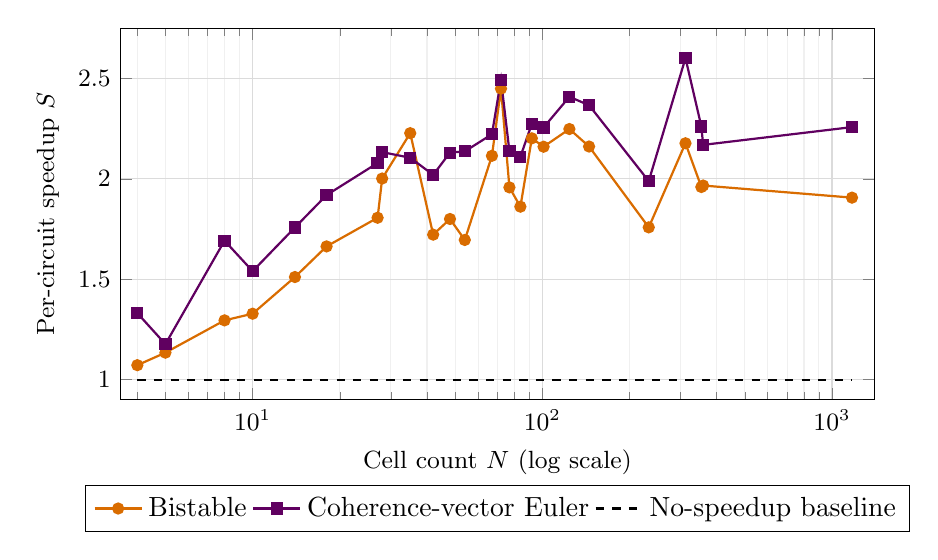
\begin{tikzpicture}
\begin{axis}[
  width=.92\linewidth,height=6.3cm,
  xmode=log,log basis x=10,
  xmin=3.5,xmax=1400,ymin=.9,ymax=2.75,
  xlabel={Cell count $N$ (log scale)},ylabel={Per-circuit speedup $S$},
  grid=both,minor grid style={gray!12},major grid style={gray!28},
  legend style={at={(0.5,-0.23)},anchor=north,legend columns=3},
  mark size=1.8pt,tick label style={font=\small},label style={font=\small}
]
\addplot[orange!85!black,thick,mark=*] coordinates {
 (4,1.072179) (5,1.134534) (8,1.295361) (10,1.328495) (14,1.511097)
 (18,1.663604) (27,1.806245) (28,2.001559) (35,2.227509) (42,1.722184)
 (48,1.800084) (54,1.695621) (67,2.114657) (72,2.449345) (77,1.957494)
 (84,1.861422) (92,2.201776) (101,2.159966) (124,2.248010) (145,2.160974)
 (233,1.758451) (312,2.177177) (354,1.959417) (359,1.966734) (1172,1.906435)
};
\addplot[violet!75!black,thick,mark=square*] coordinates {
 (4,1.331397) (5,1.176958) (8,1.692164) (10,1.540245) (14,1.758061)
 (18,1.919137) (27,2.078879) (28,2.133035) (35,2.105155) (42,2.019538)
 (48,2.130735) (54,2.136783) (67,2.222140) (72,2.493300) (77,2.137483)
 (84,2.109861) (92,2.274065) (101,2.255751) (124,2.408614) (145,2.366550)
 (233,1.988613) (312,2.601277) (354,2.260629) (359,2.169131) (1172,2.257614)
};
\addplot[black,dashed,thick] coordinates {(4,1) (1172,1)};
\legend{Bistable,Coherence-vector Euler,No-speedup baseline}
\end{axis}
\end{tikzpicture}
\caption{hfut-sim 25电路逐电路加速比折线。两条曲线均来自相同的5次配对中位计时。}
\label{fig:scaling-line}
\end{figure}

hfut Coherence预实验采用$\Delta t=10^{-16}\,\mathrm{s}$、总时长$4.096\times10^{-12}\,\mathrm{s}$，即40960个内部时间步，并非默认约700000步的长时配置。该缩短协议适合等价回归与早期性能筛查，不能替代最终长时动态实验。图~\ref{fig:preliminary}仅比较两个数据集的套件总时间加速比；最终稿应由至少30次重复的逐电路箱线图替换。

\begin{figure}[H]
\centering
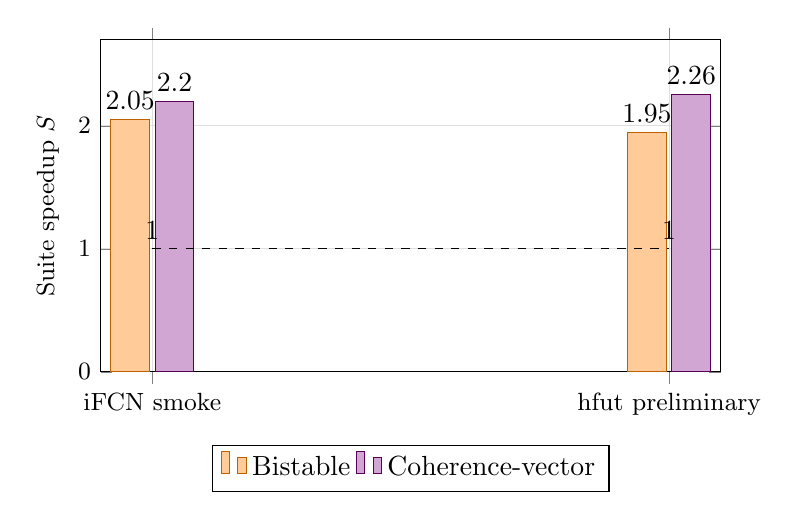
\begin{tikzpicture}
\begin{axis}[
  width=.78\linewidth,height=5.8cm,
  ybar,bar width=14pt,
  ymin=0,ymax=2.7,
  ylabel={Suite speedup $S$},
  symbolic x coords={iFCN smoke,hfut preliminary},
  xtick=data,
  nodes near coords,legend style={at={(0.5,-0.22)},anchor=north,legend columns=2},
  grid=major,
  major grid style={gray!25},
  tick label style={font=\small},label style={font=\small}
]
\addplot[fill=orange!40,draw=orange!75!black] coordinates
  {(iFCN smoke,2.050483) (hfut preliminary,1.946164)};
\addplot[fill=violet!35,draw=violet!70!black] coordinates
  {(iFCN smoke,2.199192) (hfut preliminary,2.256771)};
\legend{Bistable,Coherence-vector}
\addplot[black,dashed,sharp plot,update limits=false]
  coordinates {(iFCN smoke,1) (hfut preliminary,1)};
\end{axis}
\end{tikzpicture}
\caption{两个开发数据集的Release套件总时间加速比；smoke与preliminary的工作量不同，不作跨数据集优劣比较。}
\label{fig:preliminary}
\end{figure}

\section{创新点、消融与局限}

\subsection{可用于SCI论证的创新点}

\begin{enumerate}
  \item \textbf{面向执行轨迹等价的稀疏物理编译。}已有空间划分常只强调渐近加速；本文额外恢复基准邻居顺序、更新顺序和浮点累加顺序，使数据结构优化具有可证明的数值护栏。
  \item \textbf{同构稀疏编译格式支撑两种物理内核。}Bistable和Coherence-vector分别生成具有相同有序耦合带布局的专用内核，同时保留各自的固定点与动态积分语义；本文不把两个后端误写成共享同一个可变运行时对象。
  \item \textbf{针对QCA四相控制的动态公共核融合。}将时钟区缓存与$\operatorname{hypot}$、$\tanh$公共子表达式复用联合起来，在不增大时间步长、不改变积分器的情况下减少Coherence-vector热循环开销。
  \item \textbf{正确性门控的性能实验方法。}逐位、逐样本比对先于计时；任一电路失败即停止汇总加速比，避免用波形视觉相似代替物理仿真一致性。
  \item \textbf{布局布线到仿真的无保存衔接。}GUI临时快照把内存设计安全接入统一解析器和两个物理引擎，解决算法生成版图必须先手工保存的工程断点。
\end{enumerate}

SCI消融实验应依次启用：仅空间桶、空间桶+有序\csr{}、再加确定性调度表、再加四相时钟缓存、最后加入Coherence公共核融合。每一步同时测编译时间、运行时间、缓存未命中、分支数和L1/L2缓存指标；不能只给总加速比。

\subsection{局限}

\begin{itemize}
  \item 严格位级等价依赖相同编译器浮点策略和硬件数学库；跨平台更合理的目标可能是预注册容差下的数值等价。
  \item 稀疏图编译增加$\mathcal O(N+M)$内存，小电路或只运行一次的布局可能看不到端到端收益。
  \item 目前不改变积分时间步，也不做事件跳步，因此Coherence-vector的渐近时间复杂度未降低。
  \item 为保持Gauss--Seidel语义，Bistable不能直接对相邻元胞并行；安全的图着色并行会改变更新轨迹，应作为独立近似或数值等价版本研究。
  \item 布局几何、作用半径、层间距或介电参数改变后必须重新编译扭结能图；不能错误复用旧缓存。
  \item 当前61个布局的结果属于开发验证；每电路30次以上重复、默认长时Coherence配置、统计显著性和完整复现包尚为\pending。
\end{itemize}

\section{英文SCI题目与摘要候选}

\subsection*{Title}

\begin{quote}
\centering\textbf{Strictly Equivalent Sparse-Compiled Acceleration of\\
Bistable and Coherence-Vector QCA Simulation}
\end{quote}

备选副标题：
\begin{center}
\textit{Order-Preserving Spatial Compilation and Four-Phase Kernel Fusion\\
for Quantum-Dot Cellular Automata}
\end{center}

\subsection*{Abstract}

\begin{quote}\small
Bistable and coherence-vector simulation of quantum-dot cellular automata (QCA) repeatedly traverses a radius-limited electrostatic interaction graph, while conventional implementations incur quadratic graph construction, pointer-heavy neighborhood access, and redundant clock and transcendental-function evaluations. This paper presents a strictly equivalent sparse-compiled acceleration framework for both physical engines. An order-preserving spatial-bucket compiler enumerates exactly the cell pairs admitted by the original three-dimensional radius test and stores their kink energies and state references in contiguous CSR-like coupling bands. The bistable backend retains the deterministic Gauss--Seidel schedule, nonlinear polarization response, and convergence criterion. The coherence-vector backend retains steady-state initialization and the selected Euler or existing component-wise Runge--Kutta path, while caching the four clock phases and fusing common \texttt{hypot} and \texttt{tanh} expressions. We establish trace equivalence by induction over neighbor accumulation, cell-update order, fixed-point iterations, and time samples. Development tests cover 61 unique QCA layouts with zero logic and numerical errors. On the 25-circuit hfut-sim preliminary protocol, the bistable and Euler coherence-vector suite speedups are $1.9462\times$ and $2.2568\times$, respectively. The coherence experiment uses a shortened non-default 40,960-step protocol; at least 30 repeated runs and the default long-duration study remain \texttt{RESULT\_PENDING}. An automatic temporary-QCA snapshot also enables direct simulation of unsaved routed layouts without changing project-file semantics.
\end{quote}

\section{结论}

本文方案的价值不在于牺牲精度换取一条近似波形，而在于把第六章的局部耦合与时钟分区思想落实为两个原物理引擎共享的稀疏编译层。Bistable保持确定性Gauss--Seidel轨迹，Coherence-\allowbreak vector保持时间网格与积分分支；空间桶、有序\csr{}、四相缓存和公共表达式融合只消除重复工作。61个布局的开发预验证支持“执行轨迹等价且存在常数级加速”这一工程判断，但正式SCI结论仍必须等待30次以上重复、默认长时Coherence实验和消融结果替换所有\pending{}标记。

\end{document}
